\documentclass{article}
\usepackage{graphicx} % Required for inserting images
\usepackage{listings} % Required for insertion of code
\usepackage{amsmath} % Required for math features
\usepackage{hyperref} % Required for adding hyperlinks
\usepackage{booktabs} % Required for better table formats
% \usepackage{geometry}\geometry{margin=1in}
\usepackage{placeins} % Required to use \FloatBarrier to ensure figures are shown before section ends
\usepackage{amssymb} % Required for math symbols
\usepackage{algorithm}
\usepackage{algpseudocode}

\title{CMOR 421 Homework 4: GPUs}
\author{Hubert King}
\date{April 26th, 2024}
\begin{document}
\maketitle

\section*{Problem 1: Reduction}
We optimize reduction code with vector of size $2^{22}=4194304$ and $128$ threads per block. 

We implement Version 2 which has each thread sum two elements (rather than one) from global memory prior to storing them in shared memory. Version 1 has a runtime of approximately 9.28 milliseconds while Version 2 has a runtime of around 5.48 milliseconds, indicating that Version 2 is just under two times faster.

We implement a Version 0 where every each thread accumulates the values from the next $n$ elements, where $n$ doubles on each iteration. This version is slower because the conditional \verb|tid % (2*s) == 0|
causes warp divergence, where threads within the same warp engage in different control paths. GPUs with divergent threads handle each control path serially, causing more idle threads and thus hindered performance.

\subsection*{Profiling}
% We compute the Arithmetic Intensity (I). Each thread performs up to two operations:
% \begin{itemize}
%     \item An addition of two elements loaded from the global memory.
%     \item Participates in a series of additions during the reduction phase within the block.
% \end{itemize}
% The total FLOPs per block can be estimated as:
% \[
% \text{FLOPs per block} = 2 \times \text{blockDim.x} - 1
% \]
% Each thread reads two elements and writes one element back (the final reduced value of the block):
% \begin{itemize}
%     \item Reads: $2 \times 4$ bytes per thread (assuming single-precision floats).
%     \item Writes: $4$ bytes per block for the final result.
% \end{itemize}
% Thus, the total data transferred per block is:
% \[
% \text{Bytes per block} = \text{blockDim.x} \times 8 + 4
% \]
% Thus,
% \[
% \text{I} = \frac{2 \times \text{blockDim.x} - 1}{8 \times \text{blockDim.x} + 4} \text{ FLOPs/byte} = 0.24\text{FLOPs/byte}
% \]
Using nvprof, we record \verb|dram_read_throughput|, \verb|dram_write_throughput|, and \verb|flop_count_sp|. 
We compute
\[
\text{bytes transferred} = (\text{dram\_read\_throughput} + \text{dram\_write\_throughput}) \times \text{runtime}
\]
and
\[
\text{Computational Intensity} = \frac{\text{flop\_count\_sp}}{\text{bytes transferred}}
\]
The following computational intensities (CI) were computed:
\[
CI_{reduction_0} = 0.2121 \text{FLOPs/byte}
\]
\[
CI_{reduction_1} = 0.2125 \text{FLOPs/byte}
\]
\[
CI_{reduction_2} = 0.2187 \text{FLOPs/byte}
\]
Performance of Versions 0, 1, and 2 are visualized in the following roofline plot.
\begin{figure}
    \centering
    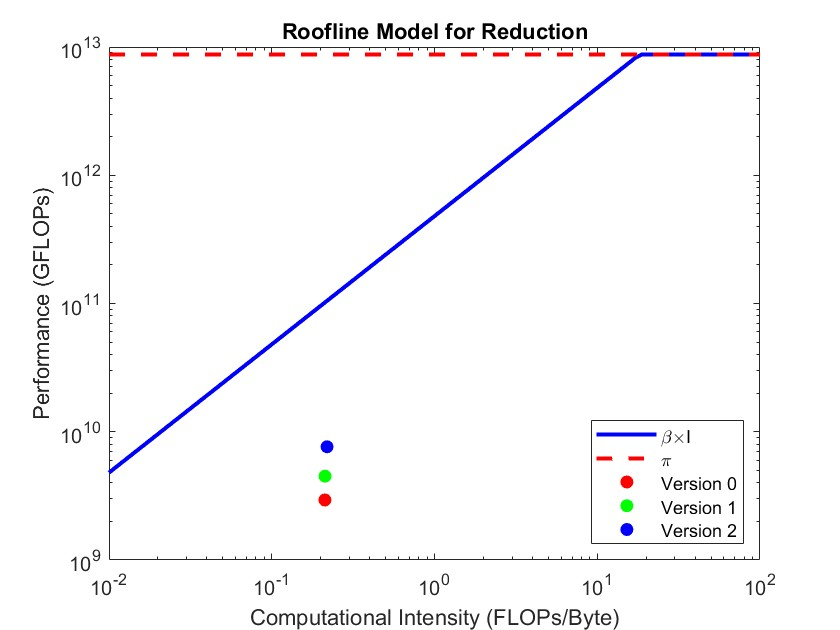
\includegraphics[height=10cm]{roofline_reduction.jpg}
    \caption{Roofline plot for Reduction Versions 0, 1, and 2.}
    \label{fig:enter-label}
\end{figure}


\section*{Problem 2: Stencil}
We consider the following iteration applied to vector $x$ with $n$ elements:
\[
y_i=\alpha(-x_{i+1}+2x_i-x_{i-1})
\]
\[
x_0=x_1
\]
\[
x_{n+1}=x_n
\]
\[
\alpha = 1
\]
We implement a Version 1 that applies the stencil using only global memory accesses.

We implement a Version 2 that applies the stencil using shared memory, where each shared memory array stores $\text{BLOCKSIZE}+2$ entries per thread block. 

We optimize the parameter $\text{BLOCKSIZE}$ and find that the best performance occurs when $\text{BLOCKSIZE} = 128$.

\subsection*{Profiling}
The following computational intensities were computed:
\[
CI_{stencil_1} = 0.22 \text{FLOPs/byte}
\]
\[
CI_{stencil_2} = 0.32 \text{FLOPs/byte}
\]
Performance of Version 1 and Version 2 are visualized in the following roofline plot. Version 2 has higher Computational Intensity and slightly higher performance, which we attribute to the use of shared memory. Shared memory accesses exploit the cache hierarchy on GPUs, allowing for lower latency and higher bandwith than global memory accesses.
\begin{figure}
    \centering
    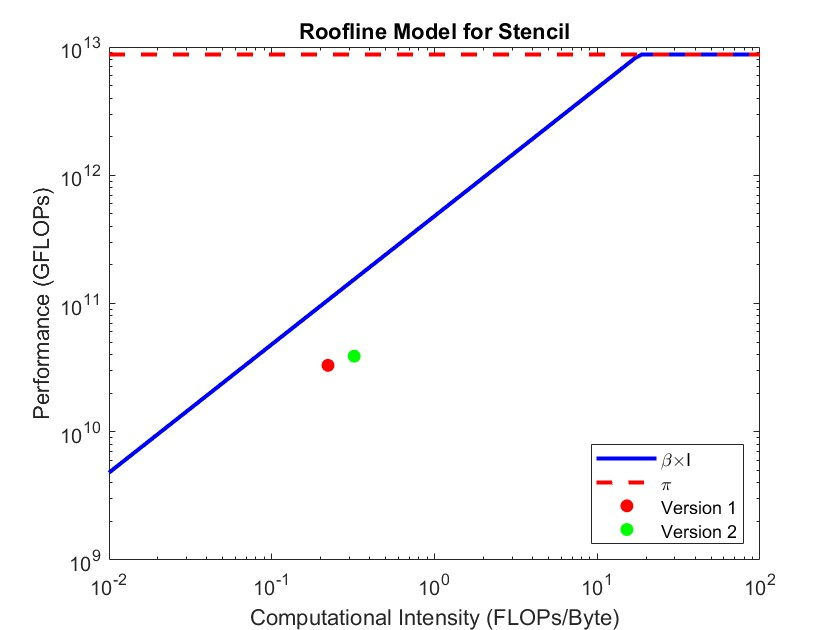
\includegraphics[height=10cm]{roofline_stencil.jpg}
    \caption{Roofline plot for Stencil Versions 1 and 2.}
    \label{fig:enter-label}
\end{figure}
\FloatBarrier


\section*{Build and Run Instructions}
Access NOTS via a login node and load the necessary modules:
\begin{verbatim}
module load purge
module load GCC/8.3.0 CUDA/10.1.168
\end{verbatim}
Verify that the module is loaded correctly and the correct version of GCC is being used:
\begin{verbatim}
module list
\end{verbatim}
Next, compile the drivers with the following command:
\begin{verbatim}
nvcc -o <executable-name> <file-name>
\end{verbatim}
To run, we use the following script, named job.slurm, which requests resources and runs the program on NOTS:
\begin{verbatim}
#!/bin/bash
#SBATCH --job-name=CMOR-421-521
#SBATCH --partition=scavenge
#SBATCH --reservation=cmor421
#SBATCH --ntasks=1
#SBATCH --mem=1G
#SBATCH --gres=gpu:1
#SBATCH --time=04:00:00
echo "My job ran on:"
echo $SLURM_NODELIST
srun <executable>
\end{verbatim}
Submit the job with the following command:
\begin{verbatim}
sbatch job.slurm
\end{verbatim}
After job completion, view the output with the following command:
\begin{verbatim}
cat slurm-<job-number>.out
\end{verbatim}
Sample output:
\begin{verbatim}
My job ran on:
bc8u27n1
Reduction with N = 4194304, blockSize = 256, numBlocks = 16384
error = 0.000000
Time to run kernel 10x:   9.28 ms.
\end{verbatim}
\end{document}
